\documentclass[letter,10pt]{article}
\usepackage[utf8]{inputenc}
\usepackage[english]{babel}
\usepackage{float}
\usepackage{graphicx}
\usepackage{caption}
\usepackage{subcaption}
\usepackage{amsmath}
\usepackage{multirow}

%opening
\title{Deep convolutional networks for quality assessment of protein folds}
\author{}

\begin{document}

\maketitle

\begin{abstract}

\end{abstract}

\section{Introduction}
% Some of this will have to be adapted to the readership of Proteins
% (It's sometimes a bit too elementary.)


The protein folding problem \cite{dill2012folding} remains one of the
outstanding challenges in structural biology. While it is usually
defined as the task of predicting the three-dimensional (3D) structure
of a protein from its amino acid sequence, it can be cast as a ranking
problem: Given a number of structural models of various quality, can
we computationally predict how close each of these models is to the
native fold of the protein?

Progress in the field is monitored through the Critical Assessment of
protein Structure Prediction (CASP) competition \cite{moult1995large},
a community-wide experiment to evaluate the accuracy of protein
folding methods at predicting protein structures ahead of their
publication. Most methods participating in the competition include a
conformational sampling step, which generates a number of plausible
protein conformations, and a quality assessment (QA) step, which
attempts to select those conformations closest to the unknown native
structure.

In this paper we explore the application of deep learning to the
problem of protein decoys quality assessment. Deep learning (DL) has
recently garnered considerable interest in the research
community \cite{lecun2015deep}, particularly in computer vision and
image recognition. Unlike more ``shallow'' machine learning
approaches, DL improves model performance by learning a hierarchical
representation of the data at hand. It alleviates the need for feature
engineering, which has traditionally constituted the bulk of the work
done by researchers.

DL has recently been applied to biological data and has yielded
remarkable results for predicting the effects of genetic variations on
human RNA splicing \cite{xiong2015human}, for identifying DNA- and
RNA-binding motifs \cite{alipanahi2015predicting}, and for predicting
the effects of non-coding DNA variants with single nucleotide
precision \cite{zhou2015predicting}. These successes have one thing in
common: they use raw data directly as input and do not attempt to
engineer features from them.

\subsection{Related work}
Deep learning methods have also been applied in the field of protein
structure quality assessment \cite{nguyen2014dlpro, cao2016deepqa,
uziela2017proq3d}. For instance, DeepQA \cite{cao2016deepqa} uses 9
scores from other QA models and 7 physico-chemical features extracted
from the structure as input features to a deep Boltzmann
machine \cite{}. In the DL-PRO algorithm \cite{nguyen2014dlpro},
authors first compute contact maps of the decoys and compress them
using PCA. The vectors from PCA are then fed into an autoencoder to
predict the score of the decoy. The authors that apply the deep
learning methods use them as the ordinary 'shallow' classifiers.
Therefore they do not get all the advantages these new techniques
offer.

More in line with the ``end-to-end'' spirit of deep learning, methods
using as input a 3D representation of the structure have been
developed to score protein-ligand
poses \cite{ragoza2017ligandscoring}, to predict ligand-binding
protein pockets \cite{jimenez2017deepsite}, or to predict the effect
of a mutation \cite{torng2017}.
% Say something about what is bad and what is good about them.


\section{Materials and Methods}

\subsection{Datasets}
<<<<<<< Updated upstream
% 
We train and assess our method using the protein decoy datasets from
the CASP competition \cite{moult2014critical}.  We use the CASP7 to
CASP10 data as training set and the CASP11 data as test set, for a
total of 564 target structures in the training set and 83 target
structures in the test set. Each target from the training set has 282
decoys on average.
%
The test dataset is split into two subsets \cite{kryshtafovych2015}:
``stage~1'' with 20 decoys per target selected randomly from all
server predictions, and ``stage~2'' with the 150 decoys per target
considered best by the Davis-QAconsensus evaluation
method \cite{kryshtafovych2015}.
%
The native structures were not included in the analysis, neither
during the training phase nor during the testing phase. To make the
structural data more consistent, the side chains of all decoy
structures were optimized using the SCWRL4 program
\cite{krivov2009improved}.

Training and test datasets cover the same interval of sequences
lengths (see Fig.~S1 in Supporting Information). To ensure that the
training and test sets are significantly different, we have aligned
all test sequences against all training sequences using
blastp \cite{altschul1990basic}.  Less than 11\% of the targets in the
test set (9 out of 83) have sequence similarity with any target in the
training set (see Table~S1 in Supporting Information).

To further assess the similarity of the two datasets, we have computed
their overlap in terms of Pfam families \cite{finn2016pfam}. Pfam
families were found using HMMER \cite{finn2015hmmer} with an E-value
cutoff of 1.0 \cite{finn2016pfam}.  Accounting for targets for which
no Pfam family could be determined, approximately 25\% of the test set
targets share a family with approximately 10\% of the training set
targets (see Table~S2 in Supporting Information).

We have also compared the structures in the training and test sets
using the ECOD database \cite{cheng2014ecod}. This database provides a
five-level classification of all structures of the RCSB PDB
\cite{berman2000protein} according to the following criteria:
architecture (A-group), possible homology (X-group), homology
(H-group), topology (T-group), and family (F-group).  Since the ECOD
classification is domain-based, multi-domain protein chains can belong
to multiple A-, X-, H-, T-, or F-groups.  The higher the level two
protein domains occupy, the more structurally similar they are.
%
A summary of the overlap between the training and test sets is
presented in Fig.~\ref{Fig:summaryTable}. For each target domain in
the test set (T0759 to T0858), a black tile indicates that at least
one structure from the training set belong to the same ECOD group (A,
X, H, T, and F). (See Fig.~S2 in Supporting Information for another
representation of the overlap between the test and training sets.)

\begin{figure}[H]
    \makebox[\textwidth]{
    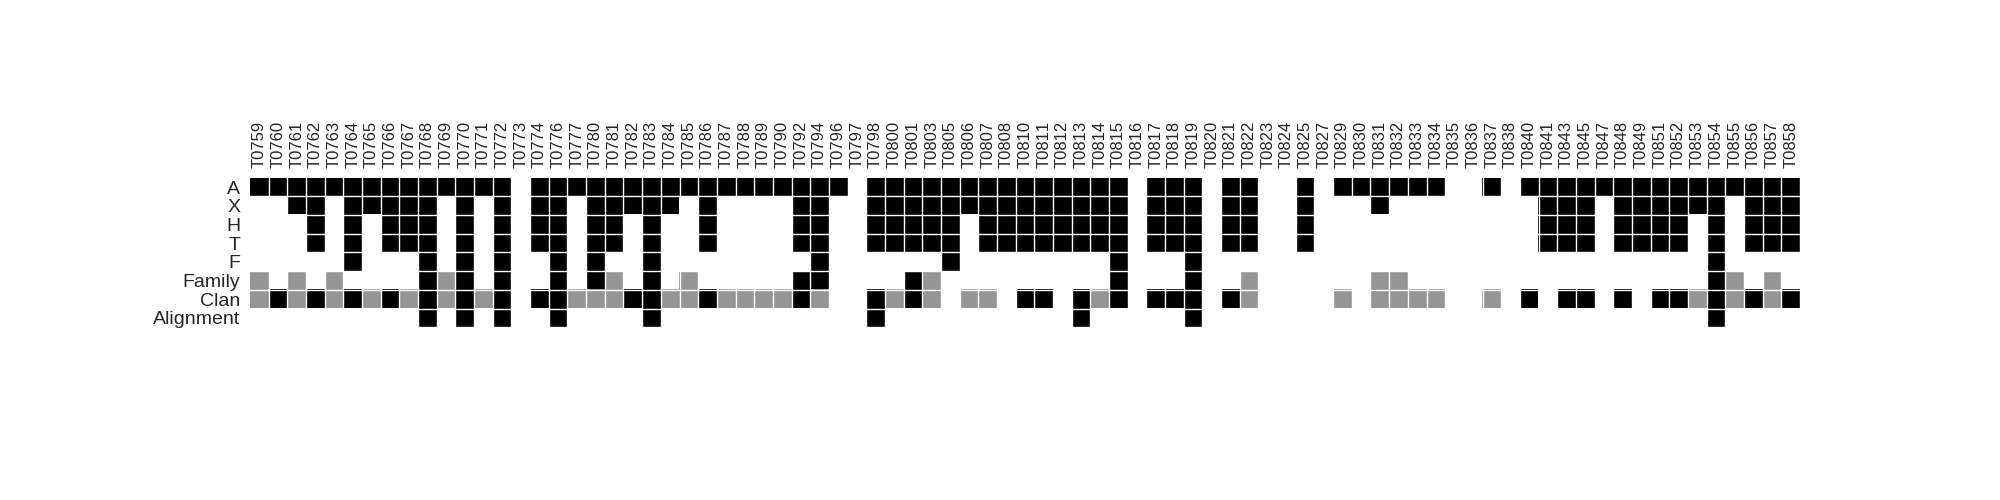
\includegraphics[width=\paperwidth]{Fig/summary_table.eps}
    }
%
    \caption{Overlap of the training set on each target domain of the
    test set (from T0759 to T0858). The first 5 rows of tiles
    correspond to the ECOD classification of protein domains (A-, X-,
    H-, T-, and F-groups). A black tile in any of these rows indicates
    that at least one structure from the training set belongs to the
    same ECOD group as the target. A white tile indicates that no
    structure belongs to the same group. Targets for which no ECOD
    classification is available are left empty (grey).
%%% GL: I see that all targets excluded from the analysis have an
%%% empty row of squares. Is T0838 excluded as well? What about the
%%% targets that are not in the list? (775, 778, 779, 791, 793, 795,
%%% 799, 802, 804, 809, 826, 828, 839, 842, 844, 846, 850) Were they
%%% all excluded from the CASP competition? The CASP11 QA paper
%%% mentions that the following targets were cancelled by the
%%% organizers: 778, 779, 791, 809, 842, 844, 846, 850. What about the
%%% other ones?
    A black tile in the ``Family'' row indicates that at least one
    structure from the training set belongs to the same Pfam family as
    the target. (Grey indicates that no Pfam family information is
    available for the target.) The ``Clan'' row shows similar
    information for Pfam clans. A black tile in the ``Alignment'' row
    indicates that at least one sequence in the training set aligns to
    the target sequence with an E-value smaller than $10^{-4}$. (Grey
    indicates that the protein structure is absent from the PDB database)}
%%% GL: You're using the code black=yes, white=no, grey=NA. I've
%%% modified the caption to reflect that.
%G: In case of alignment I skipped absent pdb structures(because I took sequences directly from structures, they are ususally shorter,
%than the sequences for predictions)
    \label{Fig:summaryTable}
\end{figure}

=======
<<<<<<< Updated upstream
%
We train and assess our method using the protein decoy datasets from
the CASP competition \cite{moult2014critical}.  We use the CASP7 to
CASP10 data as training set and the CASP11 data as test set, for a
total of 564 target structures in the training set and 83 target
structures in the test set. Each target from the training set has 282
decoys on average.
%
The test dataset is split into two subsets \cite{kryshtafovych2015}:
``stage~1'' with 20 decoys per target selected randomly from all
server predictions, and ``stage~2'' with the 150 decoys per target
considered best by the Davis-QAconsensus evaluation
method \cite{kryshtafovych2015}.
%
The native structures were not included in the analysis, neither
during the training phase nor during the testing phase. To make the
structural data more consistent, the side chains of all decoy
structures were optimized using the SCWRL4 program
\cite{krivov2009improved}.

Training and test datasets cover the same interval of sequences
lengths (see Fig.~S1 in Supporting Information). To ensure that the
training and test sets are significantly different, we have aligned
all test sequences against all training sequences using
blastp \cite{altschul1990basic}.  Less than 11\% of the targets in the
test set (9 out of 83) have sequence similarity with any target in the
training set (see Table~S1 in Supporting Information).

To further assess the similarity of the two datasets, we have computed
their overlap in terms of Pfam families \cite{finn2016pfam}. Pfam
families were found using HMMER \cite{finn2015hmmer} with an E-value
cutoff of 1.0 \cite{finn2016pfam}.  Accounting for targets for which
no Pfam family could be determined, approximately 25\% of the test set
targets share a family with approximately 10\% of the training set
targets (see Table~S2 in Supporting Information).

We have also compared the structures in the training and test sets
using the ECOD database \cite{cheng2014ecod}. This database provides a
five-level classification of all structures of the RCSB PDB
\cite{berman2000protein} according to the following criteria:
architecture (A-group), possible homology (X-group), homology
(H-group), topology (T-group), and family (F-group).  Since the ECOD
classification is domain-based, multi-domain protein chains can belong
to multiple A-, X-, H-, T-, or F-groups.  The higher the level two
protein domains occupy, the more structurally similar they are.
%
A summary of the overlap between the training and test sets is
presented in Fig.~\ref{Fig:summaryTable}. For each target domain in
the test set (T0759 to T0858), a black tile indicates that at least
one structure from the training set belong to the same ECOD group (A,
X, H, T, and F). (See Fig.~S2 in Supporting Information for another
representation of the overlap between the test and training sets.)

\begin{figure}[H]
    \makebox[\textwidth]{
    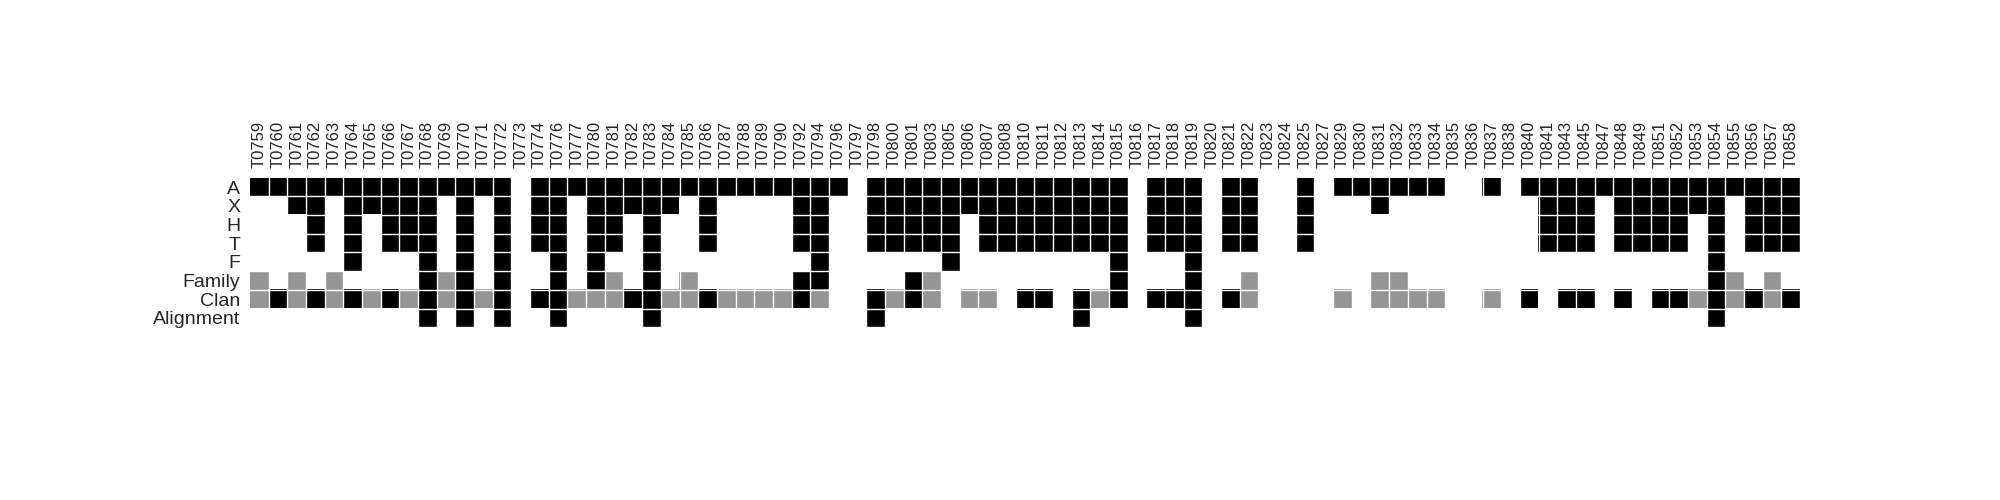
\includegraphics[width=\paperwidth]{Fig/summary_table.eps}
    }
%
    \caption{Overlap of the training set on each target domain of the
    test set (from T0759 to T0858). The first 5 rows of tiles
    correspond to the ECOD classification of protein domains (A-, X-,
    H-, T-, and F-groups). A black tile in any of these rows indicates
    that at least one structure from the training set belongs to the
    same ECOD group as the target. A white tile indicates that no
    structure belongs to the same group. Targets for which no ECOD
    classification is available are left empty (grey).
%%% GL: I see that all targets excluded from the analysis have an
%%% empty row of squares. Is T0838 excluded as well? What about the
%%% targets that are not in the list? (775, 778, 779, 791, 793, 795,
%%% 799, 802, 804, 809, 826, 828, 839, 842, 844, 846, 850) Were they
%%% all excluded from the CASP competition? The CASP11 QA paper
%%% mentions that the following targets were cancelled by the
%%% organizers: 778, 779, 791, 809, 842, 844, 846, 850. What about the
%%% other ones?
    A black tile in the ``Family'' row indicates that at least one
    structure from the training set belongs to the same Pfam family as
    the target. (Grey indicates that no Pfam family information is
    available for the target.) The ``Clan'' row shows similar
    information for Pfam clans. A black tile in the ``Alignment'' row
    indicates that at least one sequence in the training set aligns to
    the target sequence with an E-value smaller than $10^{-4}$. (Grey
    indicates that the protein structure is absent from the PDB database)}
%%% GL: You're using the code black=yes, white=no, grey=NA. I've
%%% modified the caption to reflect that.
%G: In case of alignment I skipped absent pdb structures(because I took sequences directly from structures, they are ususally shorter,
%than the sequences for predictions)
    \label{Fig:summaryTable}
\end{figure}

=======

We train and assess our method using the protein decoy datasets from
the CASP competition \cite{moult2014critical}.  We use the CASP7 to
CASP10 data as training set and the CASP11 data as test set, for a
total of 564 target structures in the training set and 83 target
structures in the test set. Each target from the training set has 282
decoys on average.
%
The test dataset is split into two subsets \cite{kryshtafovych2015}:
``stage~1'' with 20 decoys per target selected randomly from all
server predictions, and ``stage~2'' with the 150 decoys per target
considered best by the Davis-QAconsensus evaluation
method \cite{kryshtafovych2015}.
%
The native structures were not included in the analysis, neither
during the training phase nor during the testing phase. To make the
structural data more consistent, the side chains of all decoy
structures were optimized using the SCWRL4 program
\cite{krivov2009improved}.

Training and test datasets cover the same interval of sequences
lengths (see Fig.~S1 in Supporting Information). To ensure that the
training and test sets are significantly different, we have aligned
all test sequences against all training sequences using
blastp \cite{altschul1990basic}.  Less than 11\% of the targets in the
test set (9 out of 83) have sequence similarity with any target in the
training set (see Table~S1 in Supporting Information).

To further assess the similarity of the two datasets, we have computed
their overlap in terms of Pfam families \cite{finn2016pfam}. Pfam
families were found using HMMER \cite{finn2015hmmer} with an E-value
cutoff of 1.0 \cite{finn2016pfam}.  Accounting for targets for which
no Pfam family could be determined, approximately 25\% of the test set
targets share a family with approximately 10\% of the training set
targets (see Table~S2 in Supporting Information).

We have also compared the structures in the training and test sets
using the ECOD database \cite{cheng2014ecod}. This database provides a
five-level classification of all structures of the RCSB PDB
\cite{berman2000protein} according to the following criteria:
architecture (A-group), possible homology (X-group), homology
(H-group), topology (T-group), and family (F-group).  Since the ECOD
classification is domain-based, multi-domain protein chains can belong
to multiple A-, X-, H-, T-, or F-groups.  The higher the level two
protein domains occupy, the more structurally similar they are.
%
A summary of the overlap between the training and test sets is
presented in Fig.~\ref{Fig:summaryTable}. For each target domain in
the test set (T0759 to T0858), a black tile indicates that at least
one structure from the training set belong to the same ECOD group (A,
X, H, T, and F). (See Fig.~S2 in Supporting Information for another
representation of the overlap between the test and training sets.)

\begin{figure}[H]
    \makebox[\textwidth]{
    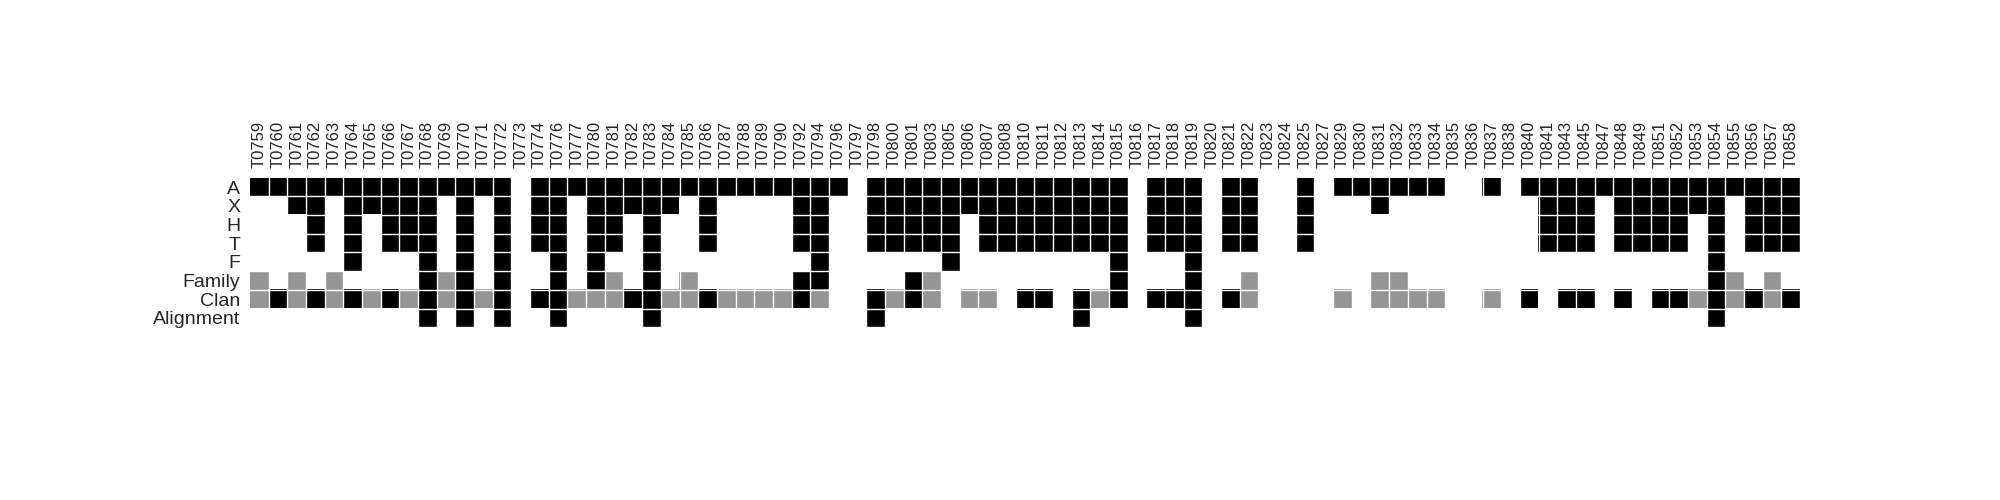
\includegraphics[width=\paperwidth]{Fig/summary_table.eps}
    }
%
    \caption{Overlap of the training set on each target domain of the
    test set (from T0759 to T0858). The first 5 rows of tiles
    correspond to the ECOD classification of protein domains (A-, X-,
    H-, T-, and F-groups). A black tile in any of these rows indicates
    that at least one structure from the training set belongs to the
    same ECOD group as the target. A white tile indicates that no
    structure belongs to the same group. Targets for which no ECOD
    classification is available are left empty (grey).
%%% GL: I see that all targets excluded from the analysis have an
%%% empty row of squares. Is T0838 excluded as well? What about the
%%% targets that are not in the list? (775, 778, 779, 791, 793, 795,
%%% 799, 802, 804, 809, 826, 828, 839, 842, 844, 846, 850) Were they
%%% all excluded from the CASP competition? The CASP11 QA paper
%%% mentions that the following targets were cancelled by the
%%% organizers: 778, 779, 791, 809, 842, 844, 846, 850. What about the
%%% other ones?
    A black tile in the ``Family'' row indicates that at least one
    structure from the training set belongs to the same Pfam family as
    the target. (Grey indicates that no Pfam family information is
    available for the target.) The ``Clan'' row shows similar
    information for Pfam clans. A black tile in the ``Alignment'' row
    indicates that at least one sequence in the training set aligns to
    the target sequence with an E-value smaller than $10^{-4}$. (Grey
    indicates that the protein structure is absent from the PDB database)}
%%% GL: You're using the code black=yes, white=no, grey=NA. I've
%%% modified the caption to reflect that.
%G: In case of alignment I skipped absent pdb structures(because I took sequences directly from structures, they are ususally shorter,
%than the sequences for predictions)
    \label{Fig:summaryTable}
\end{figure}


>>>>>>> Stashed changes
>>>>>>> Stashed changes

\subsection{Input}
% The protein structure is represented by 11 density maps corresponding
to the atom types defined in Table \ref{Tbl:atomTypes}. These atom
types are a simplification of the 20 types proposed by Huang and
Zou \cite{huang2006iterative, huang2008iterative}, to reduce the
memory footprint of the model.
%
% Type 1 = S31, S30
% Type 2 = N2N, N2X
% Type 3 = Nar
% Type 4 = N2+, N21
% Type 5 = N3+
% Type 6 = O2M, O2S
% Type 7 = O3H
% Type 8 = O2-
% Type 9 = C2+, C2-, C2M, C2S
% Type 10 = Car
% Type 11 = C3C, C3A, C3X
%
The density of an atom is modeled using the function
\begin{equation}
\label{eq:rho}
\rho(r) =  \begin{cases}
               e^{-\frac{r^2}{2}}&\text{if } r\leq 2.0\text{ \AA} \\
               0                 &\text{if } r>2.0\text{ \AA} \\
            \end{cases}
\end{equation}
The atomic density is projected to the grid corresponding to its atom
type. Each grid has a resolution of 1~\AA\ and has $120\times
120\times 120$ cells.

\begin{table}[H]
\begin{center}
\begin{tabular}{ c | l | l }
    
    Type & Description & Atoms \\
    \hline
    1 & Sulfur/selenium & CYS:SG, MET:SD, MSE:SE \\ \hline
    2 & Nitrogen (amide) & ASN:ND2, GLN:NE2, backbone N (including N-terminal) \\ \hline
    3 & Nitrogen (aromatic) & HIS:ND1/NE1, TRP:NE1 \\ \hline
    4 & Nitrogen (guanidinium) & ARG:NE/NH1/NH2 \\ \hline
    5 & Nitrogen (ammonium) & LYS:NZ \\ \hline
    6 & Oxygen (carbonyl) & ASN:OD1, GLN:OE1, backbone O (except C-terminal) \\ \hline
    7 & Oxygen (hydroxyl) & SER:OG, THR:OG1, TYR:OH \\ \hline
    8 & Oxygen (carboxyl) & ASP:OD1/OD2, GLU:OE1/OE2, \\
     & & C-terminal O, C-terminal OXT \\ \hline
    9 & Carbon (sp2) & ARG:CZ, ASN:CG, ASP:CG, GLN:CD, GLU:CD, \\
     & & backbone C \\ \hline
    10 & Carbon (aromatic) & HIS:CG/CD2/CE1, \\
     & & PHE:CG/CD1/CD2/CE1/CE2/CZ, \\ 
     & & TRP:CG/CD1/CD2/CE2/CE3/CZ2/CZ3/CH2, \\
     & & TYR:CG/CD1/CD2/CE1/CE2/CZ \\ \hline
    11 & Carbon (sp3) & ALA:CB, ARG:CB/CG/CD, ASN:CB, ASP:CB, \\
     & & CYS:CB, GLN:CB/CG, GLU:CB/CG, HIS:CB, \\
     & & ILE:CB/CG1/CG2/CD1, \\
     & & LEU:CB/CG/CD1/CD2, \\
     & & LYS:CB/CG/CD/CE, \\
     & & MET:CB/CG/CE, MSE:CB/CG/CE, \\
     & & PHE:CB, PRO:CB/CG/CD, \\
     & & SER:CB, THR:CB/CG2, \\
     & & TRP:CB, TYR:CB, VAL:CB/CG1/CG2, \\
     & & backbone CA \\ \hline    
\end{tabular}
    
    \caption {Atom types used in this work. Atoms in each group are
    identified using their standard PDB residue names and atom names.}

    \label{Tbl:atomTypes}
\end{center}
\end{table}

Figure~\ref{Fig:atomic_densities} illustrates the atomic densities for
a simple $\alpha$-helical peptide (PDB code 5eh6). This structure
contains only 6 of the 11 atom types, and only those density maps are
shown.

\begin{figure}[H]
    \centering
    \includegraphics[width=\linewidth]{Fig/Densities_V3_15cm_wide.eps}

    \caption{Representation of a protein structure (PDB code 5eh6)
    using atomic densities. The density maps are calculated according
    to Eq.~\ref{eq:rho} and rendered using Pymol \cite{PyMOL} with an
    isosurface level of $0.5$.}

    \label{Fig:atomic_densities}
\end{figure}


\subsection{Model}
% Convolutional neural networks were first proposed for image
recognition by LeCun et al.\ \cite{lecun1989backpropagation} but have
gained wider recognition after the ImageNet 2012
competition \cite{krizhevsky2012imagenet}. In this work we use 3D
convolutional networks to score protein structures. The architecture
of the model is shown in Fig.~\ref{Fig:CNNModel}.  It is comprised of
three blocks of alternating convolutional, volumetric batch
normalization, and ReLU layers, followed by three fully-connected
layers with ReLU nonlinearities. The final output of the network is a
single number, interpreted as the score of the input structure.

\begin{figure}[H]
    \centering
    \includegraphics[width=\linewidth]{Fig/ConvnetDiagramFinal_smaller.eps}

    \caption{Schematic representation of the convolutional neural
    network architecture used in this work. Line connections across
    boxes denote the consecutive application of a 3D convolutional
    layer (``Convolution''), a batch normalization layer
    (``BatchNorm''), and a ReLU layer. Arrows between boxes denote
    maximum pooling layers (``MaxPooling''). The labels ``$\times M$''
    denote the number of filters used in the corresponding 3D
    convolutional layer. The size of all filters and maximum pooling
    domains are $3\times 3\times 3$. The grey stripes denote
    one-dimensional vectors and crossed lines between them stand for
    fully-connected layers with ReLU non-linearities. Details of the
    model parameters can be found in Supporting Information Table~S4.}

    \label{Fig:CNNModel}
\end{figure}

Each 3D convolutional layer takes $N$ input density maps $f$ and
transforms them using $M$ filters $F$ according to the following
formula:
$$
f^\text{out}_i (\mathbf{r}) = \sum^{N}_{j=1} \int F_i (\mathbf{r} - \mathbf{r'}) \cdot f^\text{in}_j(\mathbf{r'}) ~d\mathbf{r'}, \quad\forall i \in [1,M]
$$
In practice, these convolutions are approximated by sums on a 3D grid.
The ReLU nonlinearity is computed as following:
$$
f^\text{out}_i (\mathbf{r}) = \begin{cases}
               f^\text{in}_i(\mathbf{r}) &\text{if } f^\text{in}_i(\mathbf{r})\geq 0\\
               0                         &\text{if } f^\text{in}_i(\mathbf{r})<0\\
            \end{cases}, \quad\forall i \in [1,M]
$$
The concept of batch normalization layer was introduced by Ioffe and
Szegedy \cite{ioffe2015batch} to address the problem of internal
covariate shift (the shift in the distribution of subnetwork outputs
during training). In practice, this layer normalizes each input value
according to the mean and variance of the corresponding input within
the subset of examples used to estimate the gradient (``batch''):
$$
\hat{f}^\text{in}_k(\mathbf{r}) = \frac{f^\text{in}(\mathbf{r}) - \mu_\text{B}}{\sqrt{\sigma^{2}_\text{B} + \epsilon}}, \quad\forall k \in [1,N_\text{B}]
$$
where $\mu_\text{B}(\mathbf{r})
= \frac{1}{N_\text{B}} \sum_{k=1}^{N_\text{B}}
f^\text{in}_i(\mathbf{r})$, and $\sigma^{2}_\text{B}
= \frac{1}{N_\text{B}} \sum_{k=1}^{N_\text{B}} \left(
f^\text{in}_i(\mathbf{r}) - \mu_\text{B}
(\mathbf{r}) \right)^2$. $N_\text{B}$ is the number of examples in the
minibatch. The constant $\epsilon = ???$ is added to avoid division by
zero. Afterwards, the output of this layer is computed by scaling the
normalized inputs:
$$
f^\text{out}_k(\mathbf{r}) = \gamma \hat{f}^\text{in}_k(\mathbf{r}) + \beta, \quad\forall k \in [1,N_B]
$$
The parameters $\gamma$ and $\beta$ are learned along with other
parameters of the network during the training.

The maximum pooling layer (``MaxPool'') is used to build a
coarse-grained representation of the input. The output of this layer
is the maximum over the cubes of size $d \times d \times d$ that cover
the input domain with the stride $l$ (distance between two consequtive
cubes along one dimension).  The output size is then approximately $l$
times smaller than the input data bounding box.  All three ``MaxPool''
layers of the model (Fig.~\ref{Fig:CNNModel}) use $d=3$ and $l=2$.

During the coarse-graining procedure, the size of the individual data
grids eventually shrinks to a single cell. The flattening layer
reshapes the array of $1\times 1\times 1$ density maps to a single
vector. Afterwards, we compute several transformations using
fully-connected layers. These layers transform a vector
$\mathbf{x}_\text{in}$ as following:
$$
\mathbf{x}_\text{out} = W \cdot \mathbf{x}_\text{in} + \mathbf{b}
$$
where $W$ is a matrix and $\mathbf{b}$ is a vector, learned during the
training. Each output vector is then transformed by a ReLU layer.


\subsection{Loss functions}

The problem of decoy quality assessment is essentially a ranking problem: we have to arrange decoys according to 
the proximity to the corresponding native structure, which is quantified using GDT score. The ranking problem 
was previously used along with neural networks to 

During the training procedure we load several decoy structures of one target (minibatch) into memory, compute the 
output of the network and the average loss:
$$ L = \frac{1}{N^{2}_B} \sum_{i=1,j=1, i \neq j}^{N_B} L_{ij} $$ 
where $N_B$ is the number of decoys in a minibatch. Afterwards, we compute the gradient of the average loss with respect 
to the network parameters and update them using Adam algorithm.

We used the margin ranking loss for each pair of decoys. Let a decoy representation be denoted as $x_i$ and therefore the output
of the network on this decoy will be $f(x_i)$. Next, let $y_{ij}$ be the ordering coefficient of the two decoys we pick:
$$
y_{ij} = \begin{cases}
               1& gdtts_i \leq gdtts_j \\
               -1& gdtts_i > gdtts_j \\
            \end{cases}
$$
Here $gdtts_i$ is the GDT score of the $i$-th decoy. In principle, any target function can be chosen. 
The pairwise ranking scoring function has the following expression:

$$ L_{ij} = w_{ij} \cdot \max \left[ 0, 1 - y_{ij} \left( f \left( x_i \right) - f \left( x_j \right) \right) \right] $$

the term $w_{ij}$ represents an example weight:

$$
w_{ij} = \begin{cases}
               1& \left| gdtts_i - gdtts_j \right| > threshold \\
               0& otherwise \\ 
            \end{cases}
$$

where the $threshold$ is a constant set to 0.1{\AA}. If the two decoys are too similar, 
we avoid scoring them against each other during the training.



\subsection{Evaluation criteria}
We evaluated our algorithm using the correlation coefficients, Z-score and loss criterions. The correlation coefficents 
were computed between the score of 
our model and GDT-TS metric for all the decoys of each target protein in a test set and then averaged. 
The Z-score is the deviation of the score of 
the best decoy for a certain protein and average decoy score for this protein:
$$ 
Z-score = \frac{f( argmin(gdtts(x_i)) ) - <f(x)>}{std.dev.f(x)}
$$ 
the best decoy is the one with the lowest GDT-TS score. 
The loss criterion is the deviation of the GDT-TS of the best decoys for a protein from the GDT-TS score of the decoy with the lowest score:
$$ 
Loss = | max_i( gdtts_i ) - gdtts( argmin(f(x_i) ) |
$$ 

\subsection{Optimization and dataset sampling}
The optimization procedure of deep convolutional networks usually is stochastic: the function value and gradient 
is estimated on a small subset (batch) of all the training 
examples. We used the batch of size 10 due to the memory limitations. Afterward the parameters of the model are 
changed in the direction of the estimated gradient.
The parameter update step was performed using the Adam algorithm \cite{}. 

The dataset was sampled in the following way: first we chose a random protein from the dataset, then we sample decoys of this protein. 
The procedure is repeated for all the 
proteins in a dataset. One pass through all the proteins in a dataset is called epoch. 
The decoys are sampled in a homogeneous way: we divide all the decoys into $M$ clusters by the value of GDT-TS score. 
Precisely, the decoy $i$ belongs to the cluster  
number $ \left[ \frac{\max(gdtts) - gdtts_i}{\max(gdtts) - \min(gdtts)} \right] + 1$, where $\max(gdtts)$ and $\min(gdtts)$ 
are computed for all the decoys of 
the chosen protein. If there are empty clusters, then we take secon decoys from each non-empty and so on until we filled the batch. 
At the end of each epoch we randomly
shuffle the order of protein and the order of decoys in each cluster. 

Each decoy from the selected batch is randomly rotated and translated. The rotations are sampled uniformly \cite{}. The translation are chosen
in such a way, that the bounding box of the translated protein lies within the box of the size 120x120x120\AA. 

To select the final model we randomly divided the training set into training and validation subsets. The validation subset consists of 
35 targets and their decoys. This subset was not sampled during the training. 
Figure \ref{Fig:TrainingLoss} shows the Kendal tau, Pearsor R coefficients and the loss on the vaidation subset. 
The final model was chosen according to the minimum loss (epoch 40).
\begin{figure}[H]
    \centering
    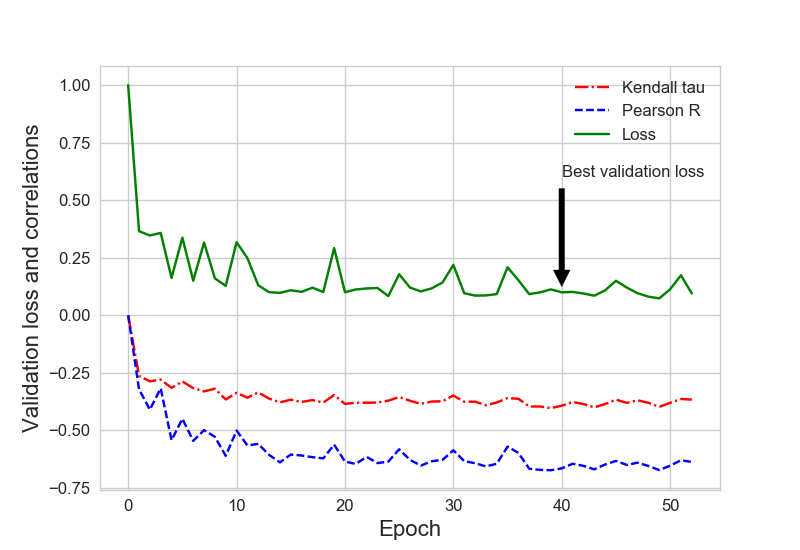
\includegraphics[width=\linewidth]{Fig/kendall_validation.png}
    \caption{The loss, Kendal tau and Pearson R coefficients evaluated on the validation subset during the training procedure. The epoch 
    denotes that all the targets in the training subset were sampled.}
    \label{Fig:TrainingLoss}
\end{figure}

The table \ref{Tbl:TrainingResults} summarizes the performance metrics on the training and validation sets for the model at epoch 40.

\begin{table}[H]
\begin{center}
\begin{tabular}{ c | c | c | c | c }
    Data subset & Loss & Pearson & Spearmann & Kendall \\
    \hline
    Training set     &0.146 &0.71 &0.61 &0.45 \\
    Validation set   &0.135 &0.71 &0.59 &0.44 \\ \hline

\end{tabular}
  \caption {Results of the model from epoch 40 on the training and validation subsets.}
    \label{Tbl:TrainingResults}
\end{center}
\end{table}

\section{Results}
During the training of the model we randomly sampled rotational and translational degrees of freedom of a decoy structure. Ideally, we 
want the score assigned by the model to a decoy to be invariant under these transformations. However Fig \ref{Fig:ScoreDistribution} 
shows that the distribution
of scores under rotations and translations follows the gaussian distribution. The Fig. \ref{Fig:DecoysScoreDistribution} 
shows the distributions of scores for several decoys. We see that the difference between the scores of different decoys is 
bigger than the variance of the score under ratations and translations. However, estimating the overlap between 
the distributions can influence the final results. Therefore, to approximate the average score of a decoy we 
sample a score under random translation and rotation 20 times for each decoy in the test set. The final score is then the average of these 
samples.

\begin{figure}[H]
    \centering
    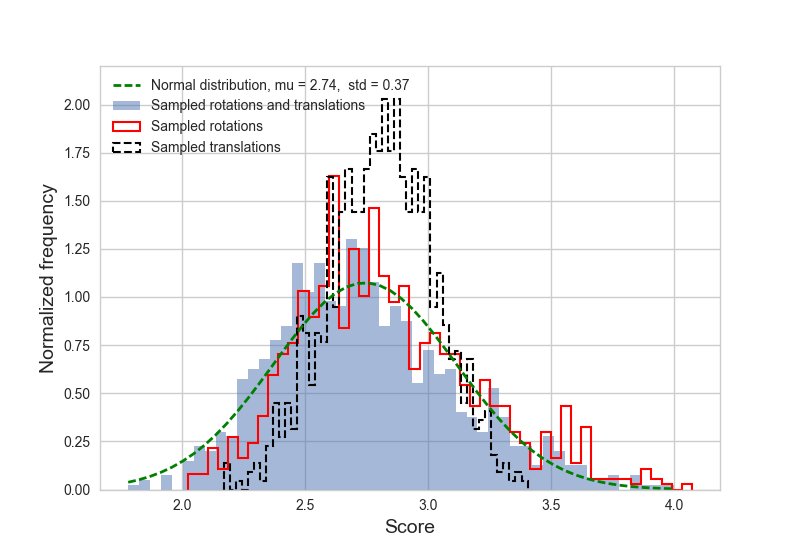
\includegraphics[width=\linewidth]{Fig/sampling_dist.png}
    \caption{The distribution of scores under random translations and rotations of the decoy 
    FALCON\_EnvFold\_TS1 for the target T0832. The distributions 
    os scores under rotations only and translations only are shown with the dashed and solid lines respectively.
    The normal distribution fitted into the sampled scores under both rotations and translations is show with the dashed line. 
    The parameters of the normal distribution are: the average $\mu = 1.38$ and the standard deviation $\sigma = 0.42$.}
    \label{Fig:ScoreDistribution}
\end{figure}

\begin{figure}[H]
    \centering
    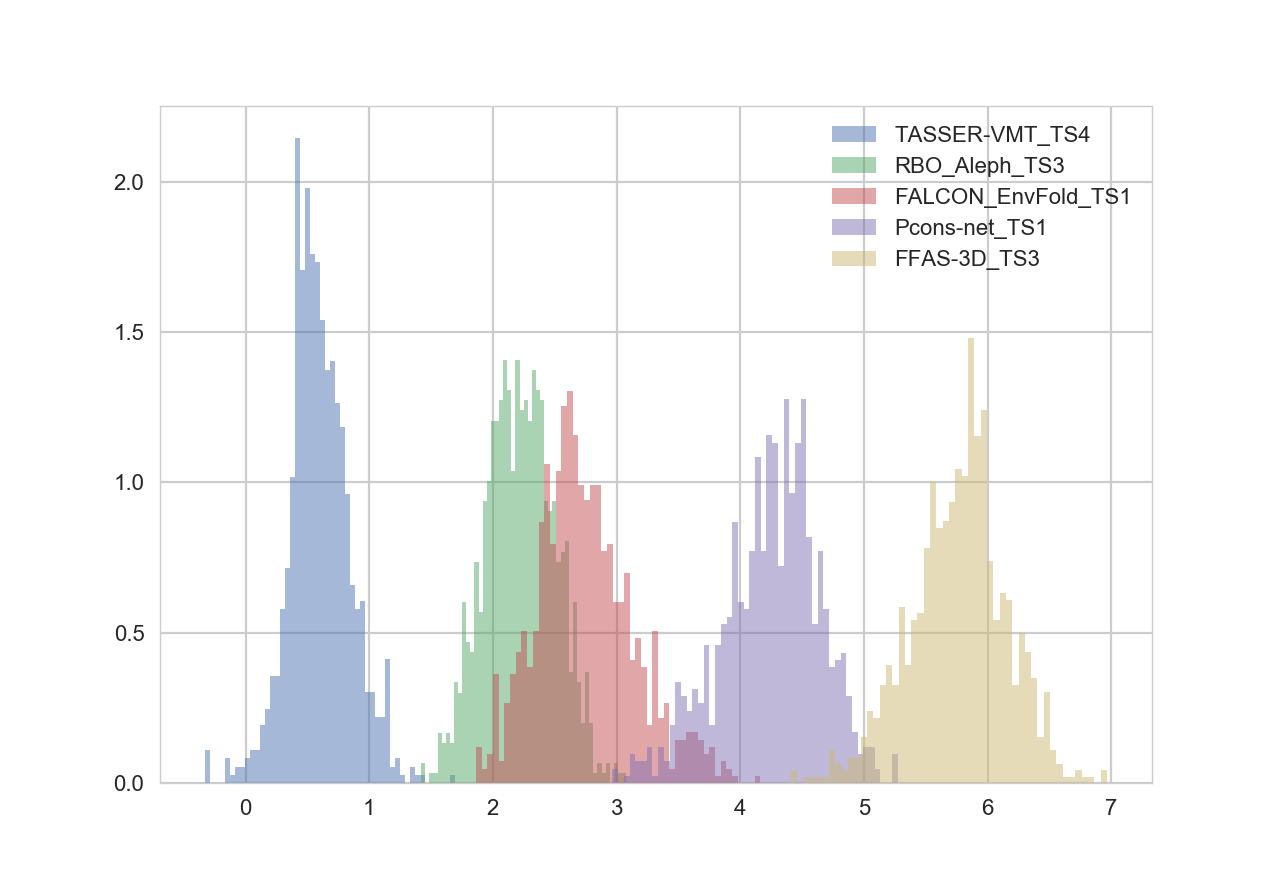
\includegraphics[width=\linewidth]{Fig/decoys_sampling_dist.png}
    \caption{The distribution of scores under random translations and rotations of several decoys for the target T0832. The 
    names arrangement from top to bottom corresponds to the increase of the score.}
    \label{Fig:DecoysScoreDistribution}
\end{figure}


Table \ref{Tbl:TestResults} shows the comparisson of our model with the state of art methods used for the decoy quality assessement. 
To evaluate the performance we used CASP11 stages 1 and 2 datasets. 
These datasets were preprocessed using SCWRL program to optimize side-chains. 

\begin{table}[H]
\begin{center}
\begin{tabular}{ c | c | c | c | c }
    \multicolumn{5}{ c }{Stage 1} \\ \hline

    QA method & Loss & Pearson & Spearmann & Kendall \\
    \hline
    \textbf{3DCNN}   &0.071 &0.528 &0.414 &0.318 \\
    ProQ2   &0.081 &0.656 &0.534 &0.408 \\
    VoroMQA &0.095 &0.621 &0.504 &0.382 \\
    Qprob   &0.097 &0.631 &0.517 &0.389 \\
    RWplus  &0.128 &0.500 &0.387 &0.291 \\ \hline
    
    \multicolumn{5}{ c }{Stage 2} \\ \hline
    
    ProQ2   &0.058 &0.372 &0.366 &0.256 \\
    \textbf{3DCNN}   &0.067 &0.420 &0.405 &0.285 \\
    Qprob   &0.068 &0.381 &0.387 &0.272 \\
    VoroMQA &0.069 &0.444 &0.437 &0.313 \\ 
    RWplus  &0.095 &0.202 &0.246 &0.175 \\ \hline

\end{tabular}
    
    \caption {Results of our method(3DCNN) and the other state-of-art quality assessment programs on the CASP11 dataset Stage 1 and 2.
            Table shows the absolute average values of correlation coefficients. The averaging was performed for each target in the 
            dataset. Afterwards all the values were averaged over all the targets.}
    \label{Tbl:TestResults}
\end{center}
\end{table}

\section{Analysis}
Deep neural networks are famous for their obscurity. The interpretation of the results obtained using these techniques can be as challenging 
as obtaining results themselves. The difficulty of interpretation brews the suspiction that the neural network learns 
artifacts in the data that correlate with the target result. In this section we attempt to show, that our network 
learns relevant description of a protein structure and does not rely on small differences in submissions between prediction groups.

First, we analyse the regions of the structures that are responsible for the decrease in its score. The method we use was proposed 
by Selvaraju R. \cite{selvaraju2016grad}. The key idea of this technique is to propagate the gradient to a certain layer and take the sum of the 
activations of this layer weighted by gradient. The weighted activation maps are then upscaled to the whole reception field of the network.
They indicate which parts of the input contributes the most to the gradient of the network output. In our case we chose the activations 
of the ReLU layer 10. The volumes of these activation maps are 25x25x25 which are the best tradeoff between interpretability and the coarsness 
of the maps. The example of the output is given on the Fig. \ref{Fig:GradCAMT0776}. 
It shows that the additional helix is not placed correctly which was detected
by the network. Also, the activations map show, that the network enforces packing: the increase in the density 
around the well packed core is penalized. Surprisingly, we found that the activation maps, obtained in the abovementioned way, 
are mostly zero for the structures close to the native ones, despite that the information about gradients was not included in 
the training procedure. 

\begin{figure}[H]
    \centering
    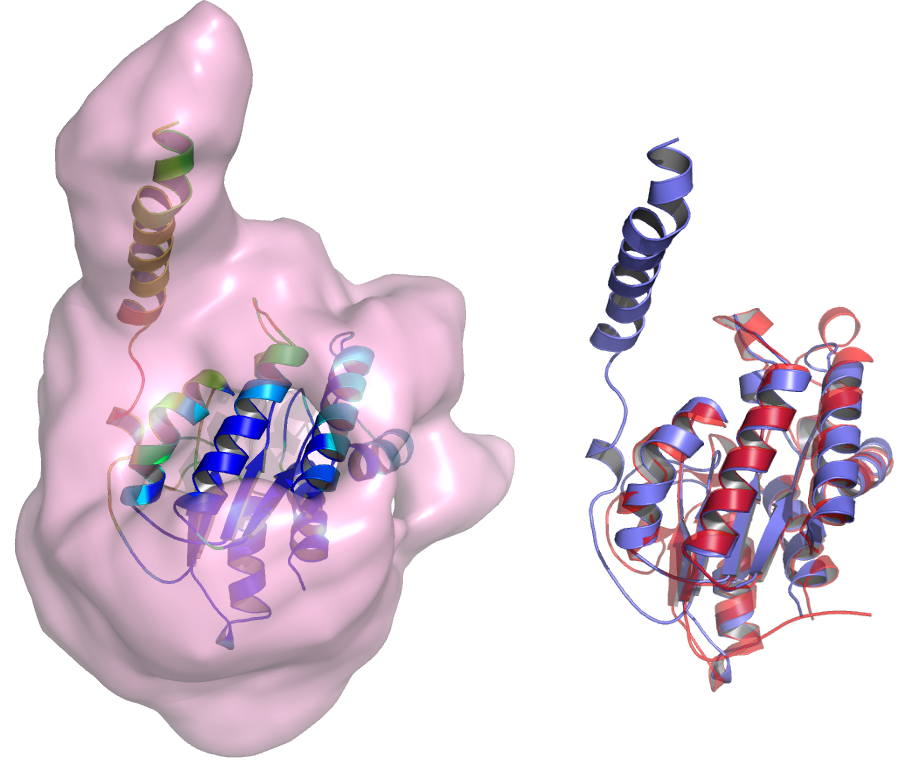
\includegraphics[width=\linewidth]{Fig/FigT0776.png}
    \caption{The scaled gradient weighted activation maps of the network (left). This example shows the candidate structure Distill\_TS3 for 
    the target T0776. On the right side the native structure (red) is aligned to the candidate (blue). The left side shows the activation 
    map with the isodurface at the level two sigma (the maps were normalized). The values of the activation map at the coordinated of protein
    atoms are shown with the color from blue to red.}
    \label{Fig:GradCAMT0776}
\end{figure}

To verify that the network we trained does not rely on artifacts in the data to rank decoys, we assessed the ranking on the dataset, designed 
by the 3DRobot algorithm \cite{deng20163drobot}. The decoys generated by this algorithm are 
uniformly distributed within RMSD range of $[0; 12\AA]$. They 
were optimized for the number of hydrogen bonds and compactness. The dataset is available online \cite{3DRobotDS}.
The absolute spearman R-coefficient averaged over all the structures in this benchmark was $0.85$, Spearman coefficient and Kendall tau were
0.83 and 0.64 respectively. The representative examples of scoring funnels are shown on the Fig \ref{Fig:3DRobotBenchmark}. 
We see, that the QA method we devised
in this work successfully ranks unrelated dataset, that has the same hyperparameters of the underlying decoys generator.

\begin{figure}[H]
    \centering
    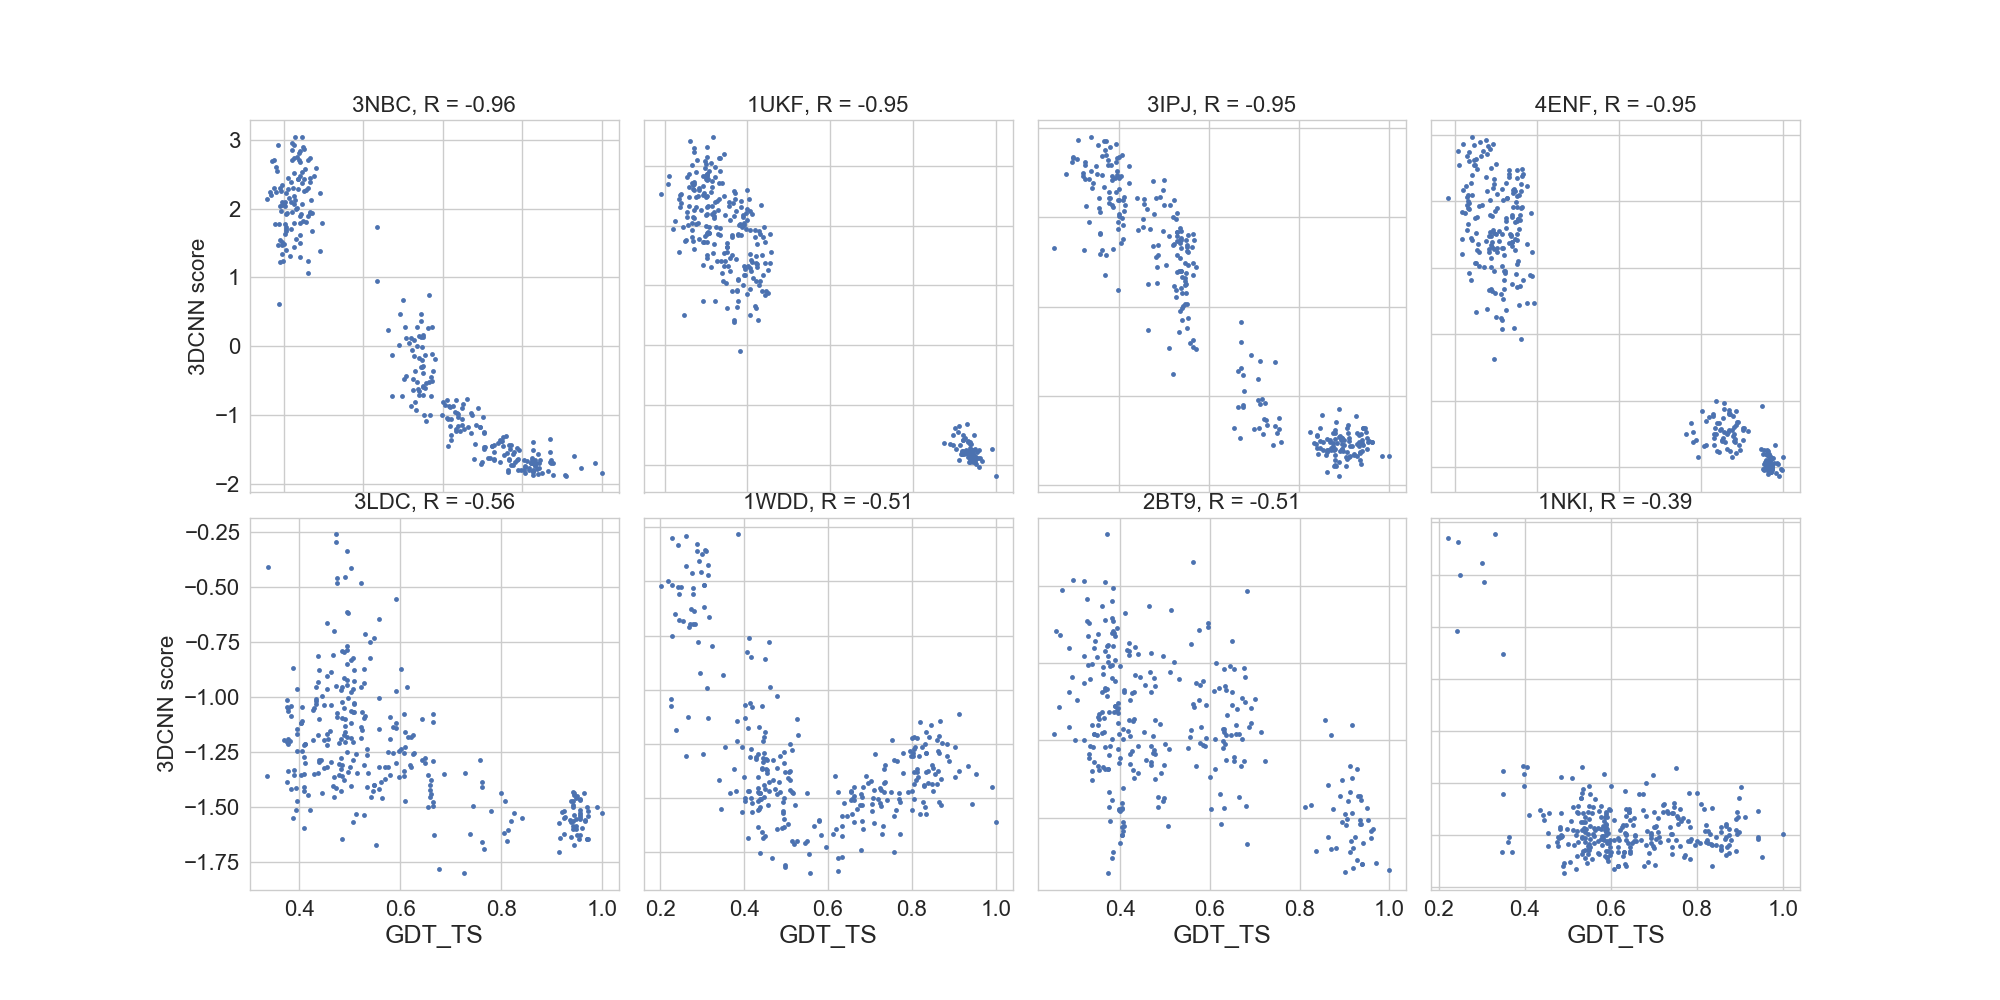
\includegraphics[width=\linewidth]{Fig/3DRobot_set_sFinal_funnels.png}
    \caption{The scoring funnels of four best correlated targets and four least correlated targets in 3DRobot benchmark.}
    \label{Fig:3DRobotBenchmark}
\end{figure}

\section{Discussion}

\bibliography{citations.bib}{}
\bibliographystyle{plain}


\end{document}
